% !TeX program = xelatex
% Compile twice with XeLaTeX; keep the assets directory beside this file.
\documentclass[UTF8,a4paper,zihao=5,fontset=fandol]{ctexart}
\usepackage[margin=23mm,top=24mm,bottom=24mm,headheight=16pt]{geometry}
\usepackage{fontspec,xcolor,graphicx,booktabs,tabularx,array,enumitem,fancyhdr,titlesec,tikz,tcolorbox,hyperref,lastpage,amsmath}
\usetikzlibrary{calc,positioning,arrows.meta}
\definecolor{Ink}{HTML}{142D4E}
\definecolor{Teal}{HTML}{294F78}
\definecolor{Muted}{HTML}{61747B}
\definecolor{Pale}{HTML}{F0F4F8}
\definecolor{Line}{HTML}{D7E3E1}
\definecolor{Gold}{HTML}{F4B544}
\hypersetup{colorlinks=true,linkcolor=Teal,urlcolor=Teal,citecolor=Teal,pdftitle={Daylight 技术设计与工程验证报告},pdfauthor={俞云烽，王宏宇}}

\setlength{\parindent}{0pt}
\setlength{\parskip}{6pt}
\linespread{1.12}
\setlist[itemize]{leftmargin=1.5em,itemsep=4pt,topsep=4pt}
\setlist[enumerate]{leftmargin=1.7em,itemsep=4pt,topsep=4pt}
\renewcommand{\arraystretch}{1.42}
\newcolumntype{Y}{>{\raggedright\arraybackslash}X}
\pagestyle{fancy}
\fancyhf{}
\fancyhead[L]{\small\sffamily\bfseries\color{Ink}DAYLIGHT\quad\normalfont\color{Muted}技术设计与工程验证}
\fancyhead[R]{\small\color{Muted}技术报告 · v1.0}
\fancyfoot[L]{\scriptsize\color{Muted}AI APPLICATION / TECHNICAL REPORT}
\fancyfoot[R]{\small\color{Teal}\thepage}
\renewcommand{\headrulewidth}{0.4pt}
\renewcommand{\footrulewidth}{0pt}
\titleformat{\section}{\LARGE\bfseries\color{Ink}}{\color{Teal}\thesection}{0.7em}{}
\titleformat{\subsection}{\large\bfseries\color{Ink}}{\thesubsection}{0.6em}{}
\titlespacing*{\section}{0pt}{0pt}{12pt}
\titlespacing*{\subsection}{0pt}{14pt}{5pt}
\tcbset{colback=Pale,colframe=Line,boxrule=.5pt,arc=2mm,left=4mm,right=4mm,top=3mm,bottom=3mm}
\newcommand{\todo}[1]{\textcolor{Teal}{【待填写：#1】}}
\newcommand{\lead}[1]{\begin{tcolorbox}\small\textbf{本章回答}\quad #1\end{tcolorbox}}
\newcommand{\placeholder}[2]{\begin{tcolorbox}[height=#2,valign=center,colback=white,colframe=Line]\centering\color{Muted}\textbf{#1}\\[5pt]\small 替换为对应参赛版本的真实图示；标注组件、边界、图例与证据来源。\end{tcolorbox}}
\newcommand{\chapterpage}[2]{\clearpage\section{#1}\lead{#2}}
\newcommand{\evidence}[1]{\par\vfill{\small\color{Muted}\textbf{交付证据}\quad #1}\par}
% 备用占位框：当前 F1–F25 均已生成，如后续新增图可暂用 \figph{图注}{高度}
\newcommand{\figph}[2]{\begin{tcolorbox}[height=#2,valign=center,colback=white,colframe=Line]
  \centering\color{Muted}\textbf{图占位\quad #1}\\[4pt]
  \small 本条图注对应的图片尚未生成，生成后按同一图注替换本占位框。图中须标组件名、数据方向、信任边界与版本。
\end{tcolorbox}}
\newcommand{\ProjectVersion}{v1.0.0}
\newcommand{\TeamName}{俞云烽，王宏宇}
\newcommand{\CommitHash}{e0ff650}
% 图片目录：从仓库根目录、本目录或 output/pdf 目录编译都能找到配图
\graphicspath{{assets/}{docs/hackathon-report/assets/}{output/pdf/assets/}}
\begin{document}
\begin{titlepage}
\begin{tikzpicture}[remember picture,overlay]
\fill[Pale] (current page.south west) rectangle (current page.north east);
\fill[Ink] (current page.south west) rectangle ($(current page.south east)+(0,17mm)$);
\fill[Gold] ($(current page.north west)+(23mm,-20mm)$) rectangle ++(15mm,1.5mm);
\end{tikzpicture}
\vspace*{5mm}
\begin{minipage}{.64\textwidth}\small\color{Ink}优刻得 AI 黑客松\\[4pt]\textbf{赛道 B · AI Application}\end{minipage}\hfill
\begin{minipage}{.28\textwidth}
\includegraphics[width=\linewidth]{ucloud-official.png}\end{minipage}
\vspace{18mm}
\begin{center}
\includegraphics[width=\textwidth]{daylight-wordmark.png}\end{center}
\vspace{6mm}
{\fontsize{26}{34}\selectfont\bfseries\color{Ink}技术设计与工程验证报告\par}
\vspace{6mm}
{\Large\color{Ink}邮件驱动的多场景 Agent 工作台\par}
\vspace{5mm}
{\color{Muted}让分散的信息，成为可追踪的下一步。\par}
\vspace{10mm}
{\color{Gold}\rule{\textwidth}{1pt}}
\vspace{5mm}
{\small\color{Muted}场景价值\quad /\quad 云原生架构\quad /\quad 可信执行\quad /\quad 可核验证据\par}
\vfill
\par\noindent\begin{tabularx}{\textwidth}{@{}p{25mm}Y@{}}\toprule
参赛团队 & \TeamName\\
项目版本 & \ProjectVersion\quad /\quad Commit：\texttt{\CommitHash}\\
文档版本 & v1.0 · 技术设计与工程验证\\
更新日期 & 2026 年 10 月 17 日\\
交付入口 &
  \href{https://github.com/why121368/Daylight}{仓库}\quad
  \href{http://192.0.2.10:3000/}{演示}\quad
  \href{https://github.com/why121368/Daylight/tree/feat/cloud-native-platform/docs/submission}{证据}\\
  \\\bottomrule

\end{tabularx}\par
\vspace{8mm}
{\footnotesize\color{Muted}统一工作区上的场景工作台：把邮件与外部回执组织成可确认的事项、待办与日程，并留下可核验的执行证据。}
\vspace{6mm}
\end{titlepage}
\pagenumbering{roman}

\section*{摘要与阅读导引}
上海科技大学校园通知高度依赖邮箱。邮件量大、时效短、入口分散时，产业报告报名、竞赛截止、材料补交与面试改期等节点容易被淹没：邮件已读，并不等于事项已办完。

Daylight 由此做成可扩展、可个性化定制的邮件管理 Agent 工作台。账号可绑定多个邮箱，并按生活、工作、校园等类别组织；日历与待办支持按单邮箱、同类别混合或全部混合查看，使不同生活场景的日程彼此隔离，减少串扰。用户按声明式模板创建场景工作台，把通知及手工补充的外部信息关联到事项，维护阶段与材料，生成待办、日程与回复草稿；写入日历或待办、对外发信与飞书会议均需人工确认。统一工作区复用邮箱、日历、RAG 与执行记录；侧栏「我的工作台 / 管理工作台」支持添加、移除与模板扩展。官方模板为智能招聘与发票助手，社区模板覆盖保研、申博与 RA、校招求职、科研投稿。

\textbf{工程亮点。}（1）\textbf{多邮箱分类隔离}：同一账号下分邮箱、分标签查看日程与待办，适配校园与生活并行的使用习惯。（2）\textbf{声明式场景工作台}：字段、阶段、识别信号与能力白名单固定在模板快照中，官方与社区模板可扩展，个人模板可导入导出，招聘等能力复用既有引擎而不复制业务代码。（3）\textbf{确认门与证据链}：建议与写入解耦，回执与「收到通知」区分；执行轨迹记录工具调用、耗时与用量，费用按历史 usage 与调用时单价核算。（4）\textbf{云原生任务拆分}：API / Worker / Scheduler 分角色部署，PostgreSQL、Redis、RabbitMQ 与对象存储协同，支持后台同步与可观测埋点。

本报告以\textbf{智能招聘}与\textbf{发票助手}为主：前者展示候选人、简历识别、筛选与邀约审核；后者展示附件发票提取、字段核对与报销准备。保研等多校申请等场景用于说明同一套平台能力的复用，不以模板数量代替业务效果。

截至 2026-10-17（Commit \texttt{e0ff650}），场景工作台本地测试 34/34、前端构建通过；云端单节点已用 Docker Compose 部署应用三角色与依赖组件，Compose 拓扑全量套件 517/517 通过。真实 QQ IMAP、对象存储与模型抽取已有联调记录，公网演示地址可达。任务排空吞吐主要受数据库提交延迟约束；证据见 \texttt{docs/submission/}。\footnote{多节点高可用、用户对照实验、业务端到端 SLA 与账单级运营成本见第 6、7 章；正文不据此外推未测结论。}

\textbf{关键词}\quad 邮件 Agent；多邮箱隔离；场景工作台；人工确认；云原生

\subsection*{评分项与章节定位}
\par\noindent\begin{tabularx}{\textwidth}{@{}p{42mm}p{13mm}Y@{}}\toprule
评分维度 & 分值 & 章节及主要证据\\\midrule
场景价值与痛点判断 & 20 & 第 1、5 章：校园邮件痛点、招聘/发票演示与边界\\
云原生架构与技术选型 & 15 & 第 2、7 章：Compose 拓扑、选型与恢复\\
Agent 能力与任务链路 & 20 & 第 3、4 章：工作台链路、确认门与审核发送\\
工程完成度与 Demo & 20 & 第 4、5、7 章：云端运行、招聘/发票实演与复现\\
成本、性能与工程分析 & 10 & 第 6 章：吞吐矩阵、埋点与 usage 计价\\
答辩现场表现 & 15 & 5 分钟汇报、3 分钟实演、7 分钟问答\\\bottomrule
\end{tabularx}\par

\subsection*{状态与数据口径}
正文按设计目标、代码实现、本地验证、真实服务联调、云端部署验证分层表述；同一 Commit 下的数字与命令以仓库证据包为准。\footnote{本地夹具结果、真实联调与多节点生产验收分层记录，不互相替代。}
\clearpage
\setcounter{tocdepth}{1}\tableofcontents
\vspace{8mm}
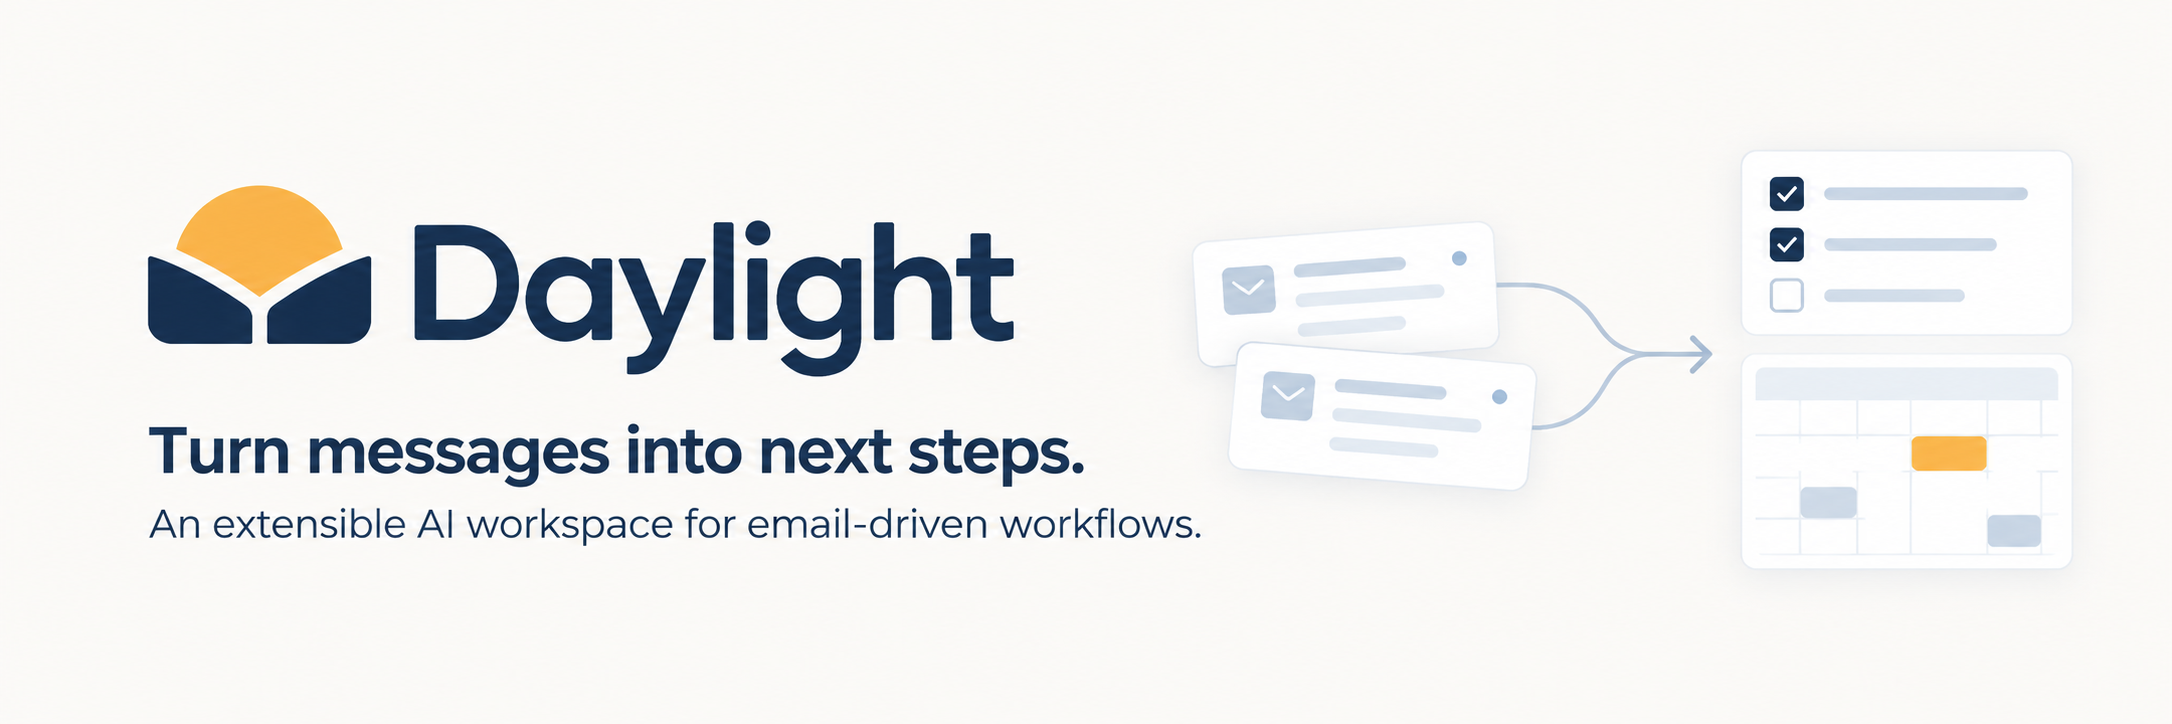
\includegraphics[width=\textwidth]{daylight-banner.png}
\clearpage\pagenumbering{arabic}

\section{场景与价值}
\lead{目标用户是谁、现有做法为何失效、Agent 工作台相对邮箱客户端增加了什么、演示主线如何选取。}

\subsection{问题从哪里来}
上海科技大学的教学、科研与校园事务大量通过邮件下达。学院通知、竞赛报名、产业报告征集、导师沟通、校招进度和发票回执往往同时到达，而且截止时间短、附件多、改期频繁。学生与协作方的常见做法是标星、建文件夹、把关键句复制到表格，或同时打开网页邮箱与系统日历。这些做法能帮助「找到那封信」，但不能稳定回答三件更重要的事：这封信属于哪一件正在进行的事、下一步该谁做、做完之后有没有留下可核对的记录。

邮件客户端把已读当作进度。已读只说明打开过正文，不说明材料已齐、场次已确认、冲突已处理或回执已发出。表格能记阶段，但与原文、附件和日历脱节，改期后旧行经常被直接覆盖，事后无法说明当时依据的是哪一封信。多邮箱并行时问题更明显：校园邮箱、个人邮箱和工作邮箱的日程混在同一个视图里，生活安排和事务截止互相遮挡。Daylight 要处理的正是这一层，而不是再提供一次对话式摘要。


\subsection{公开研究与上海科技大学校园问卷}
公开材料说明，邮件过载和「读过但没有下一步」并不是个别使用习惯。McKinsey Global Institute 对互动型知识工作者的估计是：约 28\% 的工作时间花在阅读、撰写和回复邮件上，另有约 19\% 花在查找信息，其中包括在自己的邮件里检索\footnote{McKinsey Global Institute, ``Social media's productivity payoff,'' \url{https://www.mckinsey.com/mgi/media-center/social-media-productivity-payoff}.}。高校场景更接近本项目的用户。Simpson、Branagan、Lau 与 Williams 于 2024 年在利兹大学一个大学院系所做的访谈发现：消息难以精准送到某一类学生，收件量因此变大，学生只阅读其中一小部分；重要邮件会被淹没，来自未知发件人或群发的信件更容易被跳过\footnote{J. Simpson, C. Branagan, V. Lau Cheng Von, L. Williams, ``Spamming our students? The use of email as a mass communication tool in higher education,'' \textit{Perspectives: Policy and Practice in Higher Education}, 2024, \url{https://doi.org/10.1080/13603108.2024.2440705}.}。该文转引 Education Advisory Board 2017 年的调查：54\% 的学生会选择性过滤来自院系的邮件。谢菲尔德大学的学习技能说明写得更直接：邮件仍是大学的主要沟通方式，管理不当会错过课程相关信息，并成为压力来源\footnote{University of Sheffield, ``How to manage your emails,'' \url{https://sheffield.ac.uk/study-skills/university/independent/manage-emails}.}。

上述研究的样本不是上海科技大学，也不能换成 Daylight 节省了多少时间。项目因此在本校做短问卷，核对同样的断点是否出现在目标用户身上。拟定对象为学生，以及参与招聘筛选、发票整理的协作方；拟定渠道为校园问卷与当面补访。表~\ref{tab:shanghaitech-survey} 与图~\ref{fig:shanghaitech-survey} 中的人数和百分比都是\textbf{结构占位}，正式提交前替换为实际发放人数、有效回收数和原始统计表。

\begin{table}[ht]
\centering
\small
\begin{tabularx}{\textwidth}{@{}p{8mm}Ycc@{}}
\toprule
\textbf{编号} & \textbf{上海科技大学校园问卷题项（占位）} & \textbf{有效选择} & \textbf{占比}\\
\midrule
Q1 & 过去一学期，重要通知曾被其他邮件淹没 & 63/86 & 73\%\\
Q2 & 用过标星、文件夹或表格，仍错过截止或场次 & 52/86 & 61\%\\
Q3 & 同时使用校园邮箱与个人或工作邮箱 & 46/86 & 54\%\\
Q4 & 改期或补材料后，难以找回当时依据的原信 & 58/86 & 68\%\\
Q5 & 希望先看到原文依据，再写入日程或发出邮件 & 68/86 & 79\%\\
\bottomrule
\end{tabularx}
\caption{上海科技大学校园短问卷占位结果。分母 86 为拟定有效回收数，不是已完成调查。替换时保留题项含义，并在表注写明发放时间、渠道与无效问卷的剔除规则。}
\label{tab:shanghaitech-survey}
\end{table}

\begin{figure}[ht]
\centering
\includegraphics[width=\textwidth]{额外01-痛点调查数据.png}
\caption{上海科技大学校园问卷五项痛点的选择比例。图中数据与表~\ref{tab:shanghaitech-survey} 一致，同属结构占位；正式提交前替换为实际回收结果。}
\label{fig:shanghaitech-survey}
\end{figure}

公开研究说明这类断点在高校邮件沟通中已经出现。本校问卷用来说明它是否同样发生在竞赛通知、面试改期和发票回执这些事情上。在真实回收结果写入之前，本章仍不报告节省工时或漏报下降的百分比。

\subsection{目标用户与失败代价}
面向的第一类用户是需要同时跟进多条邮件事务的在校学生和申请人。一封竞赛或面试通知被淹没，代价是错过场次或带错材料。第二类是招聘协作方：简历散落在收件箱，筛选、补问和邀约若没有统一入口，容易漏人，也容易在未核对时发出邮件。第三类是需要整理发票邮件的师生：金额、抬头和附件若只靠复制，字段错误会在报销准备阶段才暴露。

这三类用户的共同结构是：输入来自邮箱，过程跨越多天，输出必须落到待办、日程或一封经过人工确认的邮件，并且每一步都能回到原文。单纯的聊天机器人或摘要接口不保存事项阶段，也不对外部副作用负责，因此不能替代这一工作台。

\begin{figure}[ht]
\centering
\includegraphics[width=\textwidth]{图01-现有人工流程与目标闭环对照.png}
\caption{左：标星、文件夹与表格三条并行且互不引用。右：同一事项上的来源、阶段、材料版本、待办、日程与回执。图中用虚线标出「已读」不能跨越到「完成」的断点。}
\label{fig:pain}
\end{figure}

\subsection{产品定义}
Daylight 是可扩展的邮件管理 Agent 工作台。统一工作区负责邮箱、日历、待办与证据链；场景工作台用声明式模板把某一类事务组织成事项。模板描述阶段、允许的行动、前置条件和是否需要回执，核心引擎按同一套确认与写入规则执行。这样新增场景时主要增加模板与专用页面，而不是复制一套邮件同步和权限逻辑。

账号可以绑定多个邮箱，并为邮箱打上生活、工作、校园等标签。日历和待办提供三种视图：只看一个邮箱、看同一标签下的邮箱、看全部。混合视图用于需要对照的时刻，默认仍按标签把不同生活场景隔开。这是针对「校园邮箱与个人邮箱长期并行」的使用方式，而不是演示时临时加上的筛选器。

\begin{figure}[ht]
\centering
\includegraphics[width=\textwidth]{图02-多邮箱标签与视图隔离.png}
\caption{一个用户下挂多个邮箱；每个邮箱有标签；日历与待办的查询范围在「单邮箱 / 同标签 / 全部」之间切换。写操作始终落在当前选中的邮箱，不因混合视图而改写其他邮箱。}
\label{fig:mailbox}
\end{figure}

\subsection{演示主线与扩展模板}
答辩演示以官方模板\textbf{智能招聘}和\textbf{发票助手}为主线。智能招聘展示简历类邮件进入工作台、生成待确认的筛选行动，以及工作台内的 OCR、分块检索和邀约审核；发票助手展示附件字段提取、对照原件和回执阶段。社区模板包括保研、申博与 RA、校招求职和科研投稿，用来说明同一工作台可以承载其他邮件事务。模板数量本身不是价值，价值在于同一确认门、同一权限模型和同一证据链是否被复用。

\begin{table}[ht]
\centering
\small
\begin{tabularx}{\textwidth}{@{}p{28mm}YY@{}}
\toprule
\textbf{对比项} & \textbf{邮箱与手工表格} & \textbf{Daylight}\\
\midrule
组织单位 & 线程或文件夹 & 事项、候选人或票据\\
进度 & 已读、未读、星标 & 阶段、材料版本、行动状态、回执\\
日程 & 另开日历手工录入 & 确认后写入，冲突先提示\\
多邮箱 & 多个客户端来回切换 & 标签隔离，混合视图可选\\
发信 & 在客户端直接发送 & 草稿与发送分开，发送要确认\\
事后核对 & 难以还原当时依据 & 证据链保留工具名、用量与错误\\
\bottomrule
\end{tabularx}
\caption{与现有做法的差异。右列描述的是已实现的产品语义，不包含未经用户实验的时间节省比例。}
\end{table}

\subsection{Agent 带来的增量}
模型负责在给定上下文中抽取字段、判断阶段并提出下一步；规则负责限制哪些行动合法、哪些前置条件尚未满足；工具负责查询邮件、检索附件、准备草稿和写入待办或日程；人负责确认会产生外部影响的步骤。四者分开之后，系统可以在模型输出不合规时拒绝写入，也可以在用户未确认时停止在草稿。邮件正文只作为待分析的数据，其中的指令不会被当作系统命令执行。

增量具体落在三处。第一，一封信被关联到事项后，后续改期和补材料沿同一事项累计，而不是变成另一条无关摘要。第二，招聘邀约和助手起草的邮件必须经过审核卡，审核卡展示发件邮箱、全部收件人、主题和正文，并核对草稿版本。第三，每次模型调用尽量留下用量，使用户能看到这封邮件花了多少次调用、覆盖了多少封，而不是只看到一句「已分析」。

\subsection{成功标准}
工程上的成功标准是：演示主线可以在已部署的云端实例上操作；越权、重复确认和进程中断有明确结果；费用与任务状态能回到原始记录。这些项在第 5 章按证据等级列出。产品上的成功标准是用户在并行事务中更少遗漏、更快回到当时的依据。用户对照实验尚未进行，因此报告不给出节省工时或漏报下降的百分比。

\section{系统架构与技术选型}
\lead{服务如何拆分、状态放在哪里、多端如何共用同一后端，以及该结构如何承受负载、扩缩和故障。}

\subsection{多端形态}
当前可运行的主客户端是 Web 工作区，由同一套前端路由提供公开页和登录后的 \texttt{/app}。相邻的 iOS 工程使用 Capacitor，直接调用本仓库的后端和账号数据，不另起一套业务服务。服务端对移动端增加了受控的跨域来源（默认仅 \texttt{capacitor://localhost}，可用环境变量扩展）、移动 API 版本号，以及邀请参加、婉拒、撤销和助手草稿等共享接口。OAuth 回跳支持 iOS 自定义 scheme。日历仍可通过私密 ICS 订阅进 Mac 与 iPhone 的系统日历，该订阅只读，不能代替工作台里的确认写入。

桌面端的产品规划覆盖 macOS（Apple 芯片与 Intel）、Windows 和 Linux。落地页已按系统推荐对应下载项；安装包尚未作为本版本交付，因此报告把它们标为预留入口，而不是已发布客户端。Android 与鸿蒙同样只保留入口和后续接入位置。架构上的约束是：业务规则、权限和任务状态只存在于服务端，各端只负责展示、本地交互和调用同一 HTTP API。这样某一端尚未交付时，不需要在该端复制邮箱同步或发信状态机。

\begin{figure}[ht]
\centering
\includegraphics[width=\textwidth]{图03-多端接入与日历订阅.png}
\caption{Web 为已交付客户端；iOS 为已对接同一后端的独立工程；macOS 双架构、Windows、Linux 为预留桌面端；Android 与鸿蒙为后续端。所有端指向同一 API。图例区分「已交付」「已联调」「预留」。ICS 订阅画成只读旁路。}
\label{fig:clients}
\end{figure}

\begin{figure}[ht]
\centering
\includegraphics[width=\textwidth]{图04-端上职责与服务端职责.png}
\caption{端上：导航、草稿编辑、确认按钮、日历视图。服务端：认证、邮箱归属、模板执行、任务、模型与 IMAP/SMTP。箭头只允许端到 API，不允许端直接写数据库或调用邮箱协议。}
\label{fig:thin}
\end{figure}

\subsection{为什么拆成三个应用角色}
开发时可以由一个 Node 进程同时提供页面和 API，便于本地迭代。生产拓扑把三类职责拆开，是因为它们的失败方式和扩容方式不同。

API 面向用户的同步操作：登录、切换邮箱、读取工作台、确认行动、查看证据链。这些请求应当快速返回。若把整次 IMAP 同步或模型抽取放在请求线程里，一个慢邮箱会占住整个进程，页面上的其他用户也被拖住。因此 API 在需要长工作时只负责校验身份和邮箱归属，然后把任务写入数据库。

Worker 领取任务并执行。它可以按副本横向增加，用来消化同步、抽取和检查点。一个 Worker 崩溃不应导致页面不可用，也不应使未完成的任务从数据库中消失。

Scheduler 只负责「到点该为哪个邮箱入队」。它不分析邮件正文。把调度和执行放在一起时，调度循环会被一次慢同步堵住，其他邮箱的周期任务跟着延迟。拆开之后，调度器的职责是入队和退避，执行速度由 Worker 数量决定。

\begin{figure}[ht]
\centering
\includegraphics[width=\textwidth]{图05-逻辑架构.png}
\caption{浏览器与 iOS 在上，API 居中。API 之下为 PostgreSQL（权威）、Redis（会话等）、对象存储（附件）、RabbitMQ（唤醒）。Worker 与 Scheduler 位于数据库两侧。最外层为 IMAP、SMTP、OpenAI 兼容模型接口和飞书。用实线表示权威读写，用虚线表示通知和外部调用。}
\label{fig:logic}
\end{figure}

\subsection{云端部署形态}
阿里云单台 ECS（Ubuntu 22.04.5，4\,vCPU，7.5\,GiB）上，Docker Compose 一键启动 9 个服务：\texttt{api}、\texttt{worker}、\texttt{scheduler}、PostgreSQL 17.6、Redis 7.4.5、RabbitMQ 4.1.4、MinIO，以及一次性的 \texttt{migrate} 与 \texttt{minio-init}。依赖通过健康检查和「一次性任务成功」约束启动顺序，迁移或建桶失败时应用容器不会起来，因此不使用固定睡眠来假装依赖已就绪。应用容器使用只读根文件系统，并丢弃全部 Linux capabilities。

公网入口为 \texttt{http://192.0.2.10:3000/}。依赖的数据库、缓存和队列端口只绑定在宿主机回环地址，供同一台机器上的校验脚本使用，不直接对公网开放。同一主机上曾经先以 systemd 跑通过三个应用角色和宿主机上的 PostgreSQL 16、Redis、RabbitMQ；当前对外服务已改由 Compose 承载。两套部署都有独立的验证记录，下文数字分别注明来源，不把两次结果混成一次。

Kubernetes 清单已写在仓库中，用于说明目标拓扑。本版本没有在真实集群上完成滚动更新、回滚和多副本验收，因此不能把清单等同于已运行的集群。

\begin{figure}[ht]
\centering
\includegraphics[width=\textwidth]{图06-单节点容器编排部署拓扑.png}
\caption{单节点上的 9 个服务、公网 3000、回环调试端口、数据卷，以及 migrate、minio-init 对应用容器的启动依赖。标注只读根文件系统。旁注 Kubernetes 为清单已有、集群未验收。}
\label{fig:compose}
\end{figure}

\begin{figure}[ht]
\centering
\includegraphics[width=\textwidth]{图07-启动顺序.png}
\caption{从构建镜像、迁移、建桶到三个应用角色的健康检查。任一前置失败则后续不启动。}
\label{fig:boot}
\end{figure}

\subsection{技术选型与理由}
\begin{table}[ht]
\centering
\small
\begin{tabularx}{\textwidth}{@{}p{32mm}p{48mm}Y@{}}
\toprule
\textbf{选择} & \textbf{理由} & \textbf{代价}\\
\midrule
React 19 与 Vite & 工作区、日历和设置共用一套组件 & 首包偏大，长任务不能放在前端\\
Node 22 与 Express & 与现有认证、邮箱和招聘代码连续 & 需自行把长任务移出请求\\
声明式场景模板 & 新场景不改同步与权限内核 & 模板升级要有版本和白名单\\
PostgreSQL & 事务、行锁、租约代数可表达任务正确性 & 提交延迟会限制任务吞吐\\
RabbitMQ & 确认、重连成熟，适合做唤醒 & 确认与数据库更新之间仍可能重复通知\\
Redis & 会话与短时协调 & 生产故障不降级为进程内内存\\
S3 兼容存储 & 附件与简历分块可与计算分离 & 权限、删除和跨用户隔离要单独测\\
OpenAI 兼容对话接口 & 可更换供应商，要求 JSON 对象输出 & 费用和延迟随供应商变化\\
\bottomrule
\end{tabularx}
\caption{选型记录的是当前系统实际使用的组件，以及接受该组件时明确付出的代价。}
\end{table}

本地 JSON 文件仍然保留，但只用于开发和测试。生产运行时要求显式设置为 production：数据库、Redis 和对象存储故障时返回错误，不把 JSON 缓存悄悄当成权威数据。否则一次数据库中断会让进程改写旧文件，恢复后两份状态无法说明哪一份为准。

\subsection{权威状态}
业务日历、场景工作台、助手草稿和任务都以 PostgreSQL 为权威。任务入队时，任务行与 outbox 行在同一事务中写入。消息队列只负责把「有新任务」告诉 Worker。队列里的消息丢失时，Worker 仍可按数据库中的未完成任务继续领取。反过来，队列里出现重复消息时，领取逻辑必须保证只有一个执行者拿到有效租约。

同一租户的同一个邮箱在任务队列上串行。招聘改期、日程取消和再次创建若并发执行，后一封信可能先改掉前一封信尚未写入的安排。串行消除了这种顺序错误。不同邮箱之间没有这层行锁，Worker 可以并行处理，从而把吞吐建立在邮箱数量上，而不是建立在对同一邮箱的并发写上。

执行者领取任务时获得租约和代数。心跳延长租约。若进程在检查点之后被杀死，租约过期后另一个执行者可以继续。旧执行者如果在过期后才把结果写回，提交前的代数校验会拒绝这次写入。检查点与该步骤的数据库副作用使用同一次提交：步骤已经成功则再次执行时返回已保存的结果，避免把同一次确认写成两条日程。

\begin{figure}[ht]
\centering
\includegraphics[width=\textwidth]{图08-数据模型.png}
\caption{用户、会话、邮箱、标签、工作台、事项、行动、材料版本、日历事件、助手草稿、jobs、job steps、outbox。标出外键方向，以及「写路径必须带邮箱归属」的约束。}
\label{fig:er}
\end{figure}

\begin{figure}[ht]
\centering
\includegraphics[width=\textwidth]{图09-一次确认的事务边界.png}
\caption{用户确认行动时，场景状态与日历写入在同一快照事务中提交。模型调用和 SMTP 画在事务之外，并注明它们不能被数据库回滚撤销。}
\label{fig:tx}
\end{figure}

\subsection{负载从哪里来，如何扩展}
这个系统的主要负载不是页面的静态请求，而是邮箱数量乘以同步频率，再乘以模型调用。页面刷新即使增加，也不应触发新的付费抽取。因此 API 副本解决的是并发读和短写入，Worker 副本解决的是积压的同步与分析，Scheduler 保持少量实例即可，避免多个调度器对同一分钟槽位重复入队。入队使用按时间槽构造的幂等键，重复调度应得到同一次任务而不是一串新任务。

同一邮箱串行是正确性约束，也是吞吐上限的来源。若用户只有一个邮箱，增加 Worker 不能线性提高该邮箱的处理速度。若用户有多个邮箱，或实例上有多个租户，增加 Worker 才有意义。外部 IMAP、模型和 SMTP 还有各自的配额，副本数不能超过这些配额仍保持正确。自动伸缩的规则可以按队列深度来写，但本版本没有在集群上运行过自动伸缩，报告不把它写成已启用的能力。

\begin{figure}[ht]
\centering
\includegraphics[width=\textwidth]{图10-扩缩容瓶颈分层.png}
\caption{从左到右：API 并发、Worker 副本、PostgreSQL 提交、邮箱行锁、外部配额。标出本版本实测中首先饱和的是数据库提交，而不是 CPU。}
\label{fig:scale}
\end{figure}

\subsection{故障时系统应表现出的行为}
依赖中断时，接口返回明确失败，页面不显示已完成。Redis 被强行停止后，生产客户端的读写会被拒绝，而不会改用进程内存继续发会话；依赖恢复后，同一客户端可以在不重新初始化业务状态的情况下继续。对象存储不可用时，附件上传失败，招聘或发票流程停在可重试的状态，不使用空附件假装提取成功。

发信是远程副作用。连接在服务器已经接受报文之后断开时，调用方无法从本地判断对方是否收到。此时发送记录保持未知，重复点击不会再次投递，必须人工核对邮箱后再决定是否重发。飞书会议链接同样在调用前写入检查点：已经拿到链接时，后续只补写日程和草稿，不因模型后半段失败而再次建会。

邮箱若连续同步失败，调度器按终态失败次数退避，从数分钟到一小时量级，成功一次后清零。这个策略防止一个失效授权码每分钟冲击一次用户的邮箱服务。用户在页面上发起的手动同步不受退避限制，以便凭据修好后立刻重试。

\begin{figure}[ht]
\centering
\includegraphics[width=\textwidth]{图11-故障与恢复总览.png}
\caption{六条路径：进程崩溃、重复消息、数据库不可用、Redis 中断、SMTP 未知、邮箱连续失败。每条路径的终点是「可重试」「保持未知」或「拒绝」，而不是统一写成成功。}
\label{fig:fail}
\end{figure}

\section{Agent 执行链路}
\lead{任务如何拆开、工具在何处被调用、上下文如何裁剪、多步失败后停在哪一个状态。}

\subsection{链路的四层}
一次完整处理分成四层，避免把「模型说了什么」直接当成「系统已经做了什么」。

第一层是采集。Worker 按邮箱读取 IMAP，只把尚待处理的邮件交给后续步骤。已经成功处理或明确跳过的邮件不会再次抽取；失败且仍落在最近窗口内的邮件可以重试。学校邮箱在 993 端口不可达时，连接改为 143 上的强制 STARTTLS，并在对端不提供 STARTTLS 时于认证前失败，从而不发送登录命令。

第二层是理解。模型在当前有效日程和邮件正文上输出结构化结果，动作限于创建、取消和改期。输出必须是约定的 JSON。无法唯一对应到已有日程时，该封邮件失败并保留重试，而不是猜测一个事件。示例数据使用预置提取结果，界面和日志必须与真实模型调用区分。

第三层是决策。场景模板根据事项阶段决定建议是否合法。例如材料未齐时不能把事项标成已提交；招聘模板中的下一步是「在招聘引擎中筛选」，而不是直接发邀约。

第四层是执行。用户确认后才写入待办或日程。需要发信时，先持久化草稿，再由单独的发送接口在 \texttt{confirmed} 为真且版本一致时调用 SMTP。

\begin{figure}[ht]
\centering
\includegraphics[width=\textwidth]{图12-智能体四层控制流.png}
\caption{采集、理解、决策、执行四层从上到下。每层的失败出口分别回到可重试、保持原状态、待确认和未知。人工确认画在第三层与第四层之间。}
\label{fig:agent}
\end{figure}

\subsection{智能招聘}
智能招聘是演示主线之一，页面保留原有招聘能力，并从工作台的官方入口进入。流程如下。

简历类邮件先进入当前邮箱的已同步集合。用户把它关联到招聘事项，或从邮件建立新的候选人上下文。系统给出的待确认行动是进入招聘引擎做筛选。确认这一行动会记下意图和待办，不会调用 SMTP。

招聘引擎内部对附件做 OCR，对文本分块并建立可引用的检索。筛选对话必须带回引用片段，避免模型只给结论而无法对照原文。邀约邮件在引擎里生成为草稿，进入与小 D 相同的审核卡：发件人固定为当前邮箱，收件人、主题和正文可改，放弃草稿不会产生发送记录。用户在审核卡确认后，发送接口才会投递。SMTP 返回接受只表示服务器接受了本次事务，不表示候选人已读，更不表示对方已确认面试。

\begin{figure}[ht]
\centering
\includegraphics[width=\textwidth]{图13-智能招聘时序.png}
\caption{参与者：用户、Web 或 iOS、API、PostgreSQL、Worker、招聘引擎、模型、对象存储、SMTP。标出「确认筛选」与「确认发送」是两次不同的人机交互。}
\label{fig:recruit-seq}
\end{figure}

\begin{figure}[ht]
\centering
\includegraphics[width=\textwidth]{图14-招聘引擎内部数据流.png}
\caption{附件进入对象存储，文本分块进入检索，对话只消费带来源的片段，邀约草稿回到审核队列。OCR 或检索失败时候选人仍留在待处理，不生成空画像。}
\label{fig:recruit-rag}
\end{figure}

\subsection{发票助手}
发票邮件进入工作台后成为待核对事项。系统提取金额、抬头、日期等字段供复制和对照，附件仍可打开原件。用户核对之前，事项停留在待核对。进入可报销一类的证据阶段时需要回执，用来记录是谁在何时对照过哪一封邮件。读取到发票不会自动创建报销完成状态，也不会改写无关日程。

\begin{figure}[ht]
\centering
\includegraphics[width=\textwidth]{图15-发票助手数据流.png}
\caption{邮件与附件、字段提取、对照界面、回执、阶段推进。自动写入在核对之前被截断。}
\label{fig:invoice}
\end{figure}

\subsection{小 D 的工具边界}
小 D 是工作区内的助手，不是另一套业务后端。它可以使用的写相关工具限于准备能力：起草邮件、读取已有草稿、在条件满足时创建飞书会议链接并准备邀约草稿、汇总当前邮箱已经保存的邮件简报。简报不临时连接 IMAP，因此它的覆盖范围是本地已同步邮件，统计省略时会标明省略。

会议工具要求当前邮箱、受邀地址、明确的起止时间和已有的飞书配置，并检查与有效日程的冲突。没有拿到真实会议链接时不写入伪造链接。链接写入之后，若关联日程被取消或改期，发送前会拦截并要求重新核对。会议时间按北京时间解释和展示。

\begin{figure}[ht]
\centering
\includegraphics[width=\textwidth]{图16-助手工具与副作用边界.png}
\caption{工具分为只读查询和准备类写入。准备类的终点是草稿或日程，SMTP 与飞书的最终对外动作单独画在确认之后。}
\label{fig:littled}
\end{figure}

\subsection{上下文如何裁剪}
模型看到的上下文按用户、邮箱、工作台和事项逐级缩小。切换邮箱会清空当前对话的界面状态，旧请求的持久结果留在原邮箱，不会串到新邮箱的审核列表。Worker 执行任务时再次核对任务上的租户和邮箱，不使用进程里「当前选中的邮箱」这种易变状态。招聘检索只使用该候选人的附件块。跨工作台的日程重叠在确认前提示，确认时仍由用户决定是否接受该时段。

提示词里要求 JSON，并给出允许的动作集合。这是为了让非法输出在解析阶段失败。它不替代权限检查：即使模型文本里要求发送或切换到别的用户，服务端仍只执行当前登录用户、当前邮箱、当前工具白名单内的操作。

\subsection{状态机}
业务阶段、行动状态和任务执行状态分开存放。业务阶段描述事项进行到哪一步，例如待筛选或待核对。行动状态描述某一次待办、草稿或发送走到哪一步。任务状态描述 Worker 是否已领取、已检查点或已终态失败。把三者写成一个字段时，一次任务重试会把业务阶段打回，或者一次草稿放弃会被显示成邮件已发送。

行动状态至少区分：待确认、已准备草稿、发送中、已被服务器接受、对方确认、已取消、结果未知。已读邮件不进入这些状态。草稿保存不进入已被接受。未知状态不允许回到发送中，除非经过人工核对并产生一次新的、有版本号的确认。

\begin{figure}[ht]
\centering
\includegraphics[width=\textwidth]{图17-行动状态机.png}
\caption{状态与允许的迁移。未知为吸收态附近的人工态，不存在指向自动重发的边。取消保留原日程记录，改期通过替代关系连接新旧事件。}
\label{fig:sm}
\end{figure}

\subsection{多步任务中断后停在哪里}
以「确认筛选后进程退出」为例：若确认事务已经提交，恢复时看到的是已写入的待办，不会再插入第二条。以「SMTP 已发出但回执没写上」为例：记录停在未知，界面不再提供盲目重发。以「飞书已返回链接但草稿未保存」为例：检查点里已有链接，恢复时补草稿而不是再次预约。这三例分别对应数据库副作用、远程邮件副作用和远程会议副作用，恢复策略故意不同。

\begin{figure}[ht]
\centering
\includegraphics[width=\textwidth]{图18-三条中断恢复时序.png}
\caption{并排三条泳道，标出崩溃点、恢复后读取的权威记录，以及是否允许第二次外部调用。}
\label{fig:recover3}
\end{figure}

\section{异常处理与可观测性}
\lead{失败如何分类、哪些失败允许自动重试、运行中的系统如何被看见。}

\subsection{失败分类}
模型输出不是合法 JSON、动作不在允许集合内、或无法唯一对应日程时，该次理解失败，不修改事项的完成状态。这类失败可以在邮件仍处于同步窗口时重试。工具超时按错误类型决定是否重试：认证失败属于需要用户修改配置的终态倾向，短暂网络错误可以在预算内退避重试。重试预算写在任务上，而不是无限循环。

权限失败直接拒绝。读取或修改任务时同时检查租户和邮箱归属，跨用户、跨邮箱返回拒绝。并发注册、会话吊销和重复入队在并发专项里单独验证，保证后写不会覆盖先写的身份边界。

数据库事务内的失败整体回滚。场景确认与日历写入共用事务时，日历写失败则场景阶段也不前进。这个性质不能外推到 SMTP：邮件服务器不参与该事务。

\begin{table}[ht]
\centering
\small
\begin{tabularx}{\textwidth}{@{}p{32mm}YY@{}}
\toprule
\textbf{情况} & \textbf{系统行为} & \textbf{人要做什么}\\
\midrule
JSON 或语义不合格 & 不写完成态，保留重试 & 可再次同步；仍失败则看错误\\
认证或配置错误 & 终态失败并记录脱敏原因 & 修改授权码或模型配置\\
邮箱连续失败 & 指数退避，手动同步除外 & 修好后手动同步\\
进程在检查点后退出 & 租约过期后续跑，拒绝旧写入 & 无需重放已成功步骤\\
SMTP 结果不明 & 持久未知，阻断重发 & 到邮箱核对后再决定\\
数据库不可用 & 请求失败，不改 JSON 权威 & 恢复依赖后重试操作\\
Redis 中断 & 拒绝会话读写，不改用内存 & 等待恢复，不切换模式\\
\bottomrule
\end{tabularx}
\caption{异常处理按「自动收敛、等待人工、明确拒绝」三类列出。}
\end{table}

\subsection{幂等与并发}
幂等键的范围是租户加邮箱加业务键。重复点击确认、消息队列重复投递、调度器在相邻分钟重复入队，都应落到同一次有效副作用。并发领取时只有一个执行者获得租约。过期代数的写入被拒绝。八个并发确认在生产闭环检查中只产生一条日程和一条执行记录。这些结论来自带真实 PostgreSQL 的测试和校验脚本，下文按脚本来源引用，不把单次本地断言说成生产承诺。

同一邮箱串行还有一个吞吐上的后果：该邮箱队首若在退避，后面的任务会等待。这是为了避免失败重试插到新邮件之前，导致改期先于原邀请被执行。处理顺序在批处理层也按收信时间从早到晚，测试覆盖了故意打乱输入后的排序。

\subsection{可观测性}
埋点写在 HTTP、数据库查询、Redis、对象存储、模型、IMAP、消息队列、作业执行和存储提交这九类路径上。采样带原始延迟，标签会做净化，避免把邮箱地址或查询串中的凭据写进指标。缓冲区有上限；写不出去时记录丢弃次数和错误，而不是假装全部成功。三个角色的就绪检查返回各自的埋点状态。

Compose 部署下，API、Worker 和 Scheduler 的就绪检查均为正常，丢弃次数为零，下沉错误为空。这只说明当时的指标管道在写，不说明业务成功率为百分之百。业务库中的任务行仍然要单独查看：修复邮箱退避之前，真实库里曾出现相邻分钟槽位上的两次失败同步，这正是「失败邮箱每分钟重投」的现场证据。修复后的策略是退避，并在失败原因中保留有界、已脱敏的说明。

证据链页面按邮件展示模型、输入与输出 Token、调用时保存的单价和费用算式。缺少用量的调用单独计数，不用样本均价乘以全部邮件数来冒充总成本。招聘引擎里的独立操作可以查看，但不拿来稀释邮件平均成本。

\begin{figure}[ht]
\centering
\includegraphics[width=\textwidth]{图19-指标与证据链.png}
\caption{左侧为三个角色的就绪与丢弃计数，右侧为一条邮件上的调用明细。标出脱敏字段不会出现授权码。}
\label{fig:obs}
\end{figure}

\begin{figure}[ht]
\centering
\includegraphics[width=\textwidth]{图20-日志任务与证据链关系.png}
\caption{日志用于排障，任务表用于恢复，证据链用于向用户解释花费和工具。三者通过任务标识关联，互不替代。}
\label{fig:obs3}
\end{figure}

\section{效果、演示与工程完成度}
\lead{哪些结论已经在哪一级证据上成立，三分钟演示看什么，仓库如何对应到这些结论。}

\subsection{证据等级}
本报告把结论分成五级，避免把「测试通过」写成「可以上线运营」。

\begin{table}[ht]
\centering
\small
\begin{tabularx}{\textwidth}{@{}p{28mm}Y@{}}
\toprule
\textbf{等级} & \textbf{本版本中的例子}\\
\midrule
代码已实现 & API、Worker、Scheduler 分角色；模板；确认门；草稿发送\\
本地测试通过 & 场景与助手的定向测试；前端生产构建\\
真实依赖通过 & 本机或云端的 PostgreSQL、Redis、RabbitMQ、对象存储、IMAP\\
云端部署通过 & 单节点 Compose 与此前的 systemd 部署、公网入口\\
生产验收 & 本版本没有宣称达到\\
\bottomrule
\end{tabularx}
\caption{阅读后文数字时先看等级。未出现的等级表示该项尚未取得。}
\end{table}

\subsection{云端已经跑过的检查}
Compose 一键启动命令在镜像层已缓存时约 11 秒返回成功。容器内全量测试 517 项通过、0 失败、0 跳过，耗时约 71.9 秒，使用的是容器内真实数据库、Redis 和 RabbitMQ，并打开了生产依赖与并发两组门控。此前 systemd 拓扑上的全量为 507 项通过。两项数字相差来自后续增加的用例，不能把 507 解释为失败。

依赖脚本在 Compose 上的结果是：任务校验 8/8，生产闭环校验 12/12，对象存储（容器内 MinIO）14/14，真实邮件校验 9/9。真实模型使用 OpenAI 兼容接口上的 \texttt{deepseek-v4.1-flash}，该接口接受 JSON 对象输出约束。校验命令经 API 容器读取真实 QQ 邮箱 2 封邮件，并完成 1 次抽取，该次延迟约 2199\,ms。公网对存活检查、就绪检查和首页的访问均为 HTTP 200，单次约 65\,ms。依赖容器重建导致网络地址变化后，三个应用角色自行恢复并保持健康。

并发专项覆盖并发幂等入队、同邮箱队首、并发领取只有一个租约、过期写入被拒绝、检查点后崩溃不重复副作用、恢复与取消只有一个成功者、跨租户隔离、outbox 只确认一次、真实队列的重复投递、快照冲突回滚，以及并发建号与会话吊销。

这些检查回答的是「在该单节点、该版本上，工程路径是否按设计失败和恢复」。它们不回答「多活集群是否已验收」，也不回答「用户节省了多少分钟」。

\subsection{演示脚本}
现场以真实运行的云端实例为主，录屏只在网络或外部依赖中断时说明已发生过的长操作。建议顺序如下，总长约三分钟。

\begin{enumerate}
\item 使用演示账号进入工作区，切换到校园类标签，说明当前视图不包含其他标签的日程。
\item 打开智能招聘，展示一封已关联的简历邮件和一条待确认的筛选行动。确认后进入引擎，指出 OCR 与检索结果带有原文片段，并指出此时没有发送按钮被自动按下。
\item 打开一张邀约草稿的审核卡，展示收件人与正文，说明不确认就不会投递。若现场未授权发信，演示停在审核卡。
\item 打开发票助手的一封票据，展示提取字段和仍待核对的阶段。
\item 打开证据链，展示一次调用的 Token 与费用算式，以及覆盖了多少封邮件。
\end{enumerate}

若某步依赖的外部服务失败，页面应停留在错误或待处理，讲解改为指出状态，而不是改口称该步已经成功。

\begin{figure}[ht]
\centering
\includegraphics[width=\textwidth]{图21-演示故事板.png}
\caption{五格界面：标签视图、招聘待确认、审核卡、发票待核对、证据链。每格下方一句讲解词，并标注该格证明的评分点。}
\label{fig:demo}
\end{figure}

\subsection{仓库与文档}
代码仓库为 \url{https://github.com/why121368/Daylight}，分支 \texttt{feat/cloud-native-platform}，本报告对应的提交为 \texttt{e0ff650}。使用步骤在仓库根目录的 README，部署步骤在 DEPLOY。提交材料中的架构、可靠性、性能、可观测性和部署记录位于 \texttt{docs/submission/}，原始日志与性能 JSONL 与汇总表放在一起，避免只保留平均值。

\section{成本、性能与取舍}
\lead{钱花在模型的哪一次调用上，时间花在哪一段提交上，为什么当前不追求更高的任务吞吐。}

\subsection{模型费用}
单次调用的费用按该次保存的单价计算：
\[
C_i=\frac{T_{\mathrm{in},i}\,P_{\mathrm{in},i}+T_{\mathrm{out},i}\,P_{\mathrm{out},i}}{10^{6}}.
\]
总费用是所有具备完整用量和单价的调用之和。缺少用量或单价的调用记为未知，不参与样本均价，也不被当成零。历史真实调用的只读核验中，一个邮箱有 34 封邮件，其中 27 封可以完整计价，样本均价为 0.00671185 元/封；已知调用的累计金额为 0.251038 元；其余 7 封因为当时的响应没有带回完整用量，不能完整计价。另有调用次数层面的覆盖统计（该次核验为 30/40 次调用）。这些数字是用量乘以调用当时配置的单价，没有与供应商账单逐笔核对。改价不回写历史记录。

因此，报告中的「约 0.0067 元/封」只适用于该邮箱、该模型、该批邮件中已完整计价的样本。它不是所有用户的承诺价格，也不是把未知邮件按均价补齐之后的总成本。

\begin{figure}[ht]
\centering
\includegraphics[width=\textwidth]{图22-单封邮件的费用构成.png}
\caption{一封邮件上可能有多次调用。图中分开画已计价、用量缺失和确认未调用模型（记零并注明）三类，并标明招聘独立操作不进入邮件均价。}
\label{fig:cost}
\end{figure}

\subsection{任务平台的延迟与吞吐}
性能矩阵使用真实 PostgreSQL 和 RabbitMQ，业务处理函数是可控的合成负载，不调用模型。因此这组数字衡量的是任务入队、领取、提交和失败路径，不是模型的端到端回答时间。

Compose 矩阵中，1、2、4 个同进程 Worker 的排空吞吐分别为 54.89、77.93、98.36 个任务/秒。单邮箱场景为 42.46 个任务/秒。每个任务增加 25\,ms 计算后降到 23.81。百分之十的任务预设为终态失败时为 62.57。埋点打开与关闭的差异约百分之 1.9，小于该次观测极差约百分之 9.4，因而不能把埋点当成吞吐下降的原因。

同一台机器上，容器内数据库的提交延迟约为 2.252\,ms/次，大约每秒 444 次提交。每个任务大约需要 4 次已提交事务，444 除以 4 约等于 111，与 4 个 Worker 时实测的约 98 个任务/秒处于同一量级。更早的 systemd 部署使用 PostgreSQL 16.15，提交约 2.886\,ms/次，4 个 Worker 约 84 个任务/秒。两次差异与数据库版本和提交延迟同向，不能单独归因为「用了容器所以更快」或「用了容器所以更慢」。4 个 Worker 时 CPU 远未占满，内存占用大约在百兆字节量级。连接池从 5 增到 10 的差异落在噪声内。

本机笔记本上的提交可以快一个数量级，吞吐也会高一个数量级。该对照只说明云端慢在提交延迟，不把笔记本数字当作容量承诺。

\begin{figure}[ht]
\centering
\includegraphics[width=\textwidth]{图23-工作进程数与排空吞吐.png}
\caption{横轴 1/2/4 个 Worker，纵轴任务/秒。叠加一条由「提交速率除以每任务事务数」得到的上限。标注合成负载、单次测量、4\,vCPU。}
\label{fig:perf}
\end{figure}

\begin{figure}[ht]
\centering
\includegraphics[width=\textwidth]{图24-一次任务的数据库往返.png}
\caption{入队事务、领取、心跳、检查点提交。说明增加 Worker 在提交饱和后收益下降。}
\label{fig:roundtrip}
\end{figure}

\subsection{端到端延迟应如何理解}
用户能感知的同步分析延迟至少包括 IMAP、排队、模型推理和结果写入。目前有把握单独引用的模型侧样本，是云端校验中那一次真实抽取的约 2.2 秒。它是一次成功调用，不是百分位，也没有在固定邮件长度上重复足够多次。因此报告不给出「端到端 p95 为某毫秒」这种尚未按固定条件测量的数字。任务平台的每秒任务数也不能换成「每秒能分析多少封真实邮件」，因为真实路径的时间主要花在模型和邮箱服务器上。

\subsection{当前取舍}
第一，正确性优先于同邮箱并行。串行和事务使改期顺序稳定、确认不会写成两条日程，同时把单邮箱吞吐限制在队首速度。第二，远程副作用优先于自动重试。未知状态会让用户多一次核对，但避免在 SMTP 已经接受后再次投递。第三，可观测优先于极致减少数据库往返。埋点的开销落在噪声内，而提交次数本身才是吞吐上限，后续若要提高任务吞吐，应合并可合并的提交或按邮箱水平扩展，而不是先关掉确认门。第四，单节点 Compose 优先于未验收的集群。它已经能公开演示和复跑测试；多节点、备份演练和 HTTPS 证书仍是未完成项，不在本版本用架构图暗示它们已生效。

\section{复现、局限与后续}
\lead{评委如何按同一版本重做关键检查，以及哪些问题本版本明确没有解决。}

\subsection{复现条件}
\begin{table}[ht]
\centering
\small
\begin{tabularx}{\textwidth}{@{}p{32mm}Y@{}}
\toprule
\textbf{项目} & \textbf{取值}\\
\midrule
仓库 & \url{https://github.com/why121368/Daylight}\\
分支与提交 & \texttt{feat/cloud-native-platform}，\texttt{e0ff650}\\
本地运行 & 按 README 安装依赖后执行开发命令，默认本机 3000 端口\\
云端运行 & 按 DEPLOY 使用环境文件执行 Compose 一键启动\\
演示地址 & \url{http://192.0.2.10:3000/}\\
测试 & 仓库内的测试脚本；生产与并发门控由环境变量打开\\
原始结果 & \texttt{docs/submission/} 下的部署、性能与可观测性目录\\
\bottomrule
\end{tabularx}
\caption{复现时以表中的提交为准。现场若使用不同提交，应在答辩中说明差异。}
\end{table}

干净环境的顺序是：取得该提交，准备不含真实密钥的环境文件，构建并等待健康检查，执行迁移校验和任务、对象存储、生产闭环脚本，最后用浏览器完成第 5 章的演示路径。真实 IMAP 与模型校验需要评委自行提供授权，仓库和本报告不包含授权码或密钥。没有这些授权时，仍可以复跑使用真实数据库和合成外部响应的套件，但不应把该结果称作真实邮箱抽取。

\begin{figure}[ht]
\centering
\includegraphics[width=\textwidth]{图25-复现流程泳道.png}
\caption{从克隆指定提交、配置环境、启动 Compose、跑门控测试到打开演示路径。密钥只出现在环境文件，不出现在仓库。}
\label{fig:repro}
\end{figure}

\subsection{安全与隐私}
登录后的接口使用会话识别用户。邮箱凭据和模型密钥只存在于服务端配置，测试日志要求脱敏。移动端跨域来源默认收紧。ICS 订阅使用有期限的私密地址，不能凭该地址切换到其他邮箱。本报告和提交材料不粘贴真实邮件正文、授权码和 Token。

\subsection{尚未解决的问题}
多节点高可用、跨机接管、Kubernetes 上的滚动更新与回滚没有验收。数据库备份恢复和对象存储恢复没有做过演练。公网入口在验证时是 HTTP，TLS 终止和证书不在已验收范围内。用户对照实验没有做，因此场景价值停留在问题定义、流程差异和可运行闭环，没有量化到时间或错误率。模型端到端延迟只有个别真实样本，没有按输入长度和并发给出稳定分布。账单级成本没有核对。桌面安装包、Android 和鸿蒙客户端没有交付。外部日历在部分路径上已有未知结果的人工核对接口，界面尚未全部接上。

\subsection{后续计划}
优先补两类证据：一是在固定邮件样本上测量从同步到结果可见的延迟分布，二是用小样本用户对照记录遗漏和回查时间。工程上优先做备份恢复演练和 HTTPS，而不是先增加未验收的编排组件。客户端按 Web 与已联调的 iOS 稳定之后，再发布桌面端和 Android、鸿蒙，并继续只调用同一套 API。

\end{document}
